\documentclass[runningheads,envcountsame]{llncs}

\usepackage{amssymb}
\usepackage{amsmath}
\usepackage{amsfonts}

\usepackage{hyperref}
\hypersetup{
    colorlinks=true,
    linkcolor=blue,
    filecolor=magenta,      
    urlcolor=cyan
    }

\usepackage{lineno}
\usepackage{tikz}
\usepackage{graphicx}
\usepackage{thmtools}
\usepackage{thm-restate}

\title{An automaton model to succinctly represent suffix-based specifications of a distributed system}

\titlerunning{An automaton model for suffix-based specifications of a distributed system}

\author{R Keerthan\inst{1,2} \and B Srivathsan\inst{2,3} \and
  R Venkatesh\inst{1}}

  \institute{Tata Consultancy Services - Innovation Labs, Pune \\
   \email{keerthanr@tcs.com, r.venky@tcs.com} \and Chennai Mathematical Institute,
  India \\
  \email{sri@cmi.ac.in} \and CNRS, ReLaX,
  IRL 2000, Siruseri, India }


  %% Macros

  \newcommand{\xra}{\xrightarrow}
  \newcommand{\Nat}{\mathbb{N}}
  \newcommand{\Aa}{\mathcal{A}}
  \newcommand{\incl}{\subseteq}
  \newcommand{\out}{\operatorname{Out}}
  \newcommand{\proj}[1]{\mathsf{P}_{#1}}
  
  \begin{document}
  
  \maketitle

  \begin{abstract}
  Deterministic Suffix-reading Automata (DSA) were introduced recently as a  concise model for regular languages. 
  DSAs can succinctly capture formal specifications that are based on \emph{sequences} of input actions (and not just single actions). For a distributed system, specifications may further depend on combinations of input sequences seen across multiple components (ports). 
  For such systems, DSAs consider all possible interleavings, resulting in large and unreadable automata.

  In this work, we enrich DSAs to include a $\parallel$ operator in its transitions. The resulting \emph{multi-port DSAs (mDSAs)} can succinctly represent concurrent suffix-based specifications. We provide a formal operational semantics for mDSAs and prove that emptiness for mDSAs is PSPACE-complete. 
  Then, we apply our results to the analysis of Expressive Decision Tables (EDTs) -- an industry notation for specifying requirements of reactive systems. The EDT notation has been successfully deployed in various industrial settings. However, arguably, due to a complex interplay between concurrency and suffix-based conditions, the notation lacks a rigorous operational semantics. As a result, existing test generation algorithms for EDTs do not give any theoretical guarantees. Here, we provide formal operational semantics for a fragment of the EDT notation using mDSAs, and reduce EDT-test-generation to mDSA-emptiness.
  
  \end{abstract}
  
  \section{Introduction}

  % Automata are very useful. In particular in formal verification and model-based testing.

  Finite state automata are all-pervasive, adopting different roles in different contexts. In this work, we focus on the role of automata as \emph{formal models of system requirements} and their subsequent application in Model Based Testing (MBT). MBT is a paradigm in formal methods where the requirements of a system under test (SUT) are first converted to a formal model. This formal model is then used to automatically generate test cases for the SUT. There are many MBT tools (see \cite{10.1145/1353673.1353681,10.1002/stvr.456} for a survey) and in several of them, the formal model is given by some extension of finite automata. 

  %Automata can be made concise.Making automata concise is a long line of work. Different ways in which they could be made concise. In MBT this helps in writing more concise specifications. 

  Converting requirements to a Deterministic Finite Automaton (DFA) or a Non-deterministic Finite Automaton (NFA) is often cumbersome. This is because DFAs and NFAs describe low level computations which reason about individual actions. There are various ways in which automata can be made consise. In Generalized Automata~\cite{DBLP:books/lib/Eilenberg76,GIAMMARRESI1999191}, transitions contain words instead of single actions. A transition $q \xra{abb} q'$ is fired from $q$ if the word $abb$ is after the automaton reaches $q$. Therefore requirements which depend on an exact sequence of actions can be represented using generalized automata more concisely. A natural extension is to allow for regular expressions in transitions, resulting in the model of Expression Automata~\cite{10.1007/978-3-540-30500-2_15} and its deterministic variant. Deterministic Expression Automata (DEA) impose restrictions on the regular expressions that can be used: they should result in a prefix-free language, and moreover, every pair of regular expressions out of state is language disjoint. This results in DEA recognizing a subset of regular languages. On the other hand, in Expression Automata, the transitions are so powerful that the states have almost no meaning: the entire automaton can be reduced to a single state and a single transition labeled by the regular expression representing the language. For languages leading to big automata, the corresponding regular expression can be complicated and incomprehensible. The goal is to hit a sweet spot where the transition labels are not too complicated, and at the same time there are fewer states than a DFA. 

   

  Deterministic suffix-reading automata (DSAs)~\cite{DBLP:journals/corr/abs-2410-22761} are a recently introduced automaton model for regular languages. Transitions are  labeled with words (as in a generalized automaton), however, the semantics is different. A transition $q \xra{abb} q'$ is fired from $q$ if a word \emph{ending} with the suffix $abb$ is seen. When there are multiple transitions out of a state, the first transition that matches is fired. Figure~\ref{fig:dsa-examples} gives some examples of DSAs.

  \begin{figure}
  \centering
  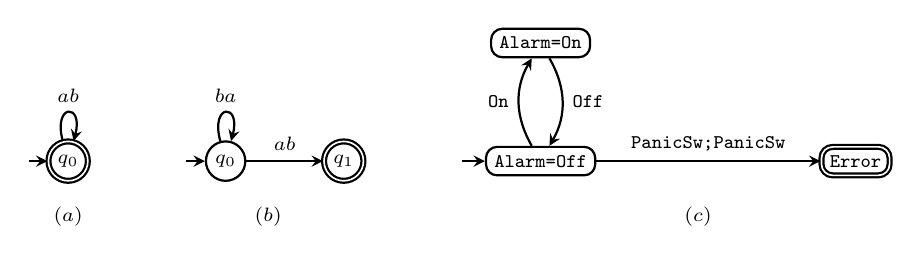
\begin{tikzpicture}[state/.style={circle, inner sep=2pt, draw, thick}]
    \begin{scope}[every node/.style={state}]
      \node [double] (0) at (0,0) {\scriptsize $q_0$};
    \end{scope}
    \begin{scope}[->, >=stealth, thick]
      \draw (-0.5, 0) to (0);
      \draw (0) to [loop above] node {\scriptsize $ab$} (0);
    \end{scope}
    \node at (0, -0.7) {\scriptsize $(a)$};

    \begin{scope}[xshift=2cm]
      \begin{scope}[every node/.style={state}]
        \node (0) at (0,0) {\scriptsize $q_0$};
        \node [double] (1) at (1.5, 0) {\scriptsize $q_1$};
      \end{scope}
      \begin{scope}[->, >=stealth, thick]
        \draw (-0.5, 0) to (0);
        \draw (0) to [loop above] node  {\scriptsize $ba$} (0);
        \draw (0) to node [above] {\scriptsize $ab$} (1);
      \end{scope}
      \node at (0.54, -0.7) {\scriptsize $(b)$};
    \end{scope}

      \begin{scope}[xshift=6cm]
        \begin{scope}
          \node [rectangle, rounded corners, draw, inner sep=3pt, thick] (0) at (0,0) {\scriptsize \texttt{Alarm=Off}};
          \node [rectangle, rounded corners, draw, inner sep=3pt, thick] (1) at (0,1.5) {\scriptsize \texttt{Alarm=On}};
          \node [rectangle, rounded corners, draw, inner sep=3pt, thick, double] (2) at (4, 0) {\scriptsize \texttt{Error}};
        \end{scope}

        \begin{scope}[->, >=stealth, thick]
          \draw (-1,0) to (0);
          \draw (0) to [bend left] node [left] {\scriptsize \texttt{On}} (1);
          \draw (1) to [bend left] node [right] {\scriptsize \texttt{Off}} (0);
          \draw (0) to node [above] {\scriptsize \texttt{PanicSw;PanicSw}} (2);
        \end{scope}
        \node at (2, -0.7) {\scriptsize $(c)$};
      \end{scope}
    
  \end{tikzpicture}
  \caption{Examples of Deterministic Suffix-reading Automata (DSA)}
  \label{fig:dsa-examples}
  \end{figure}

  In Figure~\ref{fig:dsa-examples}(a), the DSA accepts all words that end with $ab$, for instance $bab, bbab, babab$, etc. The transition $q_0 \xra{ab} q_0$ is fired as soon as a word ending with $ab$ is seen. In Figure~\ref{fig:dsa-examples}(a), we can view the state $q_0$ as tracking two suffixes $ba$ and $ab$. When $ba$ is seen before $ab$, the self-loop is triggered; otherwise when $ab$ is seen first, the transition to $q_1$ is taken. For example, on word $bbab$, the automaton starts at $q_0$, and on $bba$ it fires $q_0 \xra{ba} q_0$, reads $b$ and remains there. Since $q_0$ is non-accepting, the word is rejected. However, on $bbaab$, the run loops on $bba$ back to $q_0$, and then reads the next $ab$ to reach $q_1$, and accept. The final example Figure~\ref{fig:dsa-examples}(c) is a \emph{suffix-based specification} of a part of an automotive software: when the alarm is off, and the panic switch is pressed twice within one second, flag an error. Here, we assume there is a symbol \texttt{tick} to denote the elapse of $1$ unit of time. So, on a word \texttt{tick}; \texttt{On}; \texttt{tick} \texttt{Off}; \texttt{PanicSw}; \texttt{PanicSw}, an error should be flagged (we have added a separator symbol ; just for clarity). This specification is succinctly represented by the DSA in Figure~\ref{fig:dsa-examples}(c).

   Since transitions in a DSA wait for specific patterns to appear, DSAs are able to represent suffix-based specifications succinctly. When we consider systems with multiple components (which we call ports), the requirements can talk about different combinations of inputs. Here are two examples. 

   \begin{figure}
   \centering
   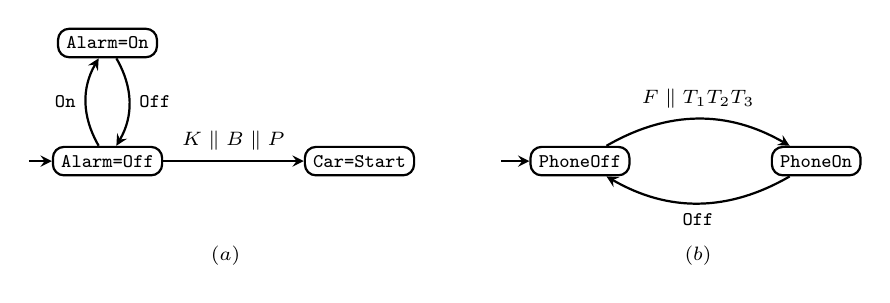
\begin{tikzpicture}
      \begin{scope}[every node/.style={rectangle, rounded corners, draw, inner sep=3pt, thick}]
        \node (0) at (0,0) {\scriptsize \texttt{Alarm=Off}};
        \node (1) at (0,1.5) {\scriptsize \texttt{Alarm=On}};
        \node (2) at (3.2,0) {\scriptsize \texttt{Car=Start}};
      \end{scope}

      \begin{scope}[->,>=stealth, thick]
        \draw (-1,0) to (0);
        \draw (0) to [bend left] node [left] {\scriptsize \texttt{On}} (1);
        \draw (1) to [bend left] node [right] {\scriptsize \texttt{Off}} (0);
        \draw (0) to node [above] {\scriptsize $K \parallel B \parallel P$} (2);
      \end{scope}

      \node at (1.5, -1.2) {\scriptsize $(a)$};

      \begin{scope}[xshift=6cm]
        \begin{scope}[every node/.style={rectangle, rounded corners, draw, inner sep=3pt, thick}]
          \node (0) at (0,0) {\scriptsize \texttt{PhoneOff}};
          \node (1) at (3,0) {\scriptsize \texttt{PhoneOn}};
        \end{scope}

        \begin{scope}[->,>=stealth, thick, auto]
          \draw (-1,0) to (0);
          \draw (0) to [bend left] node {\scriptsize $F \parallel T_1 T_2 T_3$} (1);
          \draw (1) to [bend left] node {\scriptsize \texttt{Off}} (0);
        \end{scope}

        \node at (1.5, -1.2) {\scriptsize $(b)$};


      \end{scope}
   \end{tikzpicture}
   \caption{Concurrent suffix-based specifications as multi-port DSAs}
   \label{fig:mdsa-examples}
   \end{figure}
   \paragraph*{Car Security System.} For a car to start, you need: key in ignition ($K$), brake pedal pressed ($B$), transmission in park ($P$), and no alarm triggered. The actions $K$, $B$ and $P$ can occur in any order. A DSA would need to represent this requirement using all $6$ permutations. Instead, we assume an alphabet that is distributed across different \emph{ports} -- ignition, brake pedal, transmission, and denote the concurrent actions as $K \parallel B \parallel P$. Figure~\ref{fig:mdsa-examples}(a) illustrates the enriched DSA.
  
   \paragraph*{Smartphone Lock Pattern} To unlock a phone with pattern: fingerprint verification ($F$) and drawing specific gesture with three touch points ($T_1;T_2;T_3$). This is represented as $F \parallel (T_1 T_2 T_3)$ and the enriched DSA is shown in Figure~\ref{fig:mdsa-examples}(b).
   
  In Appendix~\ref{app:examples-of-parallel}, we give many more examples of similar situations that involve multiple ports and suffix-based requirements across all of them. To the best of our knowledge, no automaton model can represent such specifications succinctly. Incorporating concurrency into the specification is paramount when requirements talk about different components of the distributed system. 
  
  \subsubsection*{Contributions.} The goal of this paper is to investigate the addition of a $\parallel$ operator into the transition syntax of DSAs. We call the resulting model as \emph{multi-port DSAs}, where the alphabet is distributed (partitioned) across multiple ports. The challenge lies in describing an operational semantics that matches with our intentions. As our first technical contribution, we provide a formal operational semantics for multi-port DSAs. 
  
  We then show that state reachability (or emptiness) for mDSAs is PSPACE-complete. For the simpler models DFAs or DSAs, reachability is linear in the input size. The higher complexity for mDSAs ties with the intuition that mDSAs can be exponentially more succinct. Our proof of PSPACE-hardness indeed exhibits such an example. 

  As our next contribution, we apply the mDSA framework to provide a formal semantics for Expressive Decision Tables (EDTs), a notation introduced by \cite{DBLP:conf/date/VenkateshSKA14} to incorporate both state-based and stream-based requirements in one convenient tabular form. The EDT notation has been successfully deployed in many industrial projects. In \cite{DBLP:conf/date/VenkateshSKA14} it has also been observed that the time and effort involved in writing EDT specifications was considerably low compared to other formalisms like  Statecharts. Many test generation tools for EDT specifications have been developed: given an EDT, and a row, the tool can generate a sequence of input actions that can trigger the input-side conditions of the particular row~\cite{DBLP:conf/enase/VenkateshSZA15a,DBLP:conf/icst/AgrawalVSZV20}. %The tricky part in the EDT notation is the use of input-output (I/O) variables that make multiple rows dependent. 
  Although EDTs have been used extensively for test generation, the notation does not yet have a formal operational semantics because of a complex interplay between concurrency and suffix-based rules. We close these gaps using the mDSA technology: we consider a fragment of the EDT notation, and map each EDT to an mDSA. This in turn gives an operational semantics for the EDT. Moreover, test generation for EDTs reduces to state reachability in mDSAs. 
  
  
  
  

  

  % Contributions. 
  % - Add a parallel operator to the syntax. Examples 2 and 3. First time that both suffix-based and concurrency have been incorporated.
  % - Challenge lies in describing an operational semantics that matches with our intentions.
  % - State reachability of mDSAs (emptiness) is PSPACE-complete. Compare with DFAs/DSAs where it is polynomial-time. This ties with the intuition that mDSAs can be exponentially more succinct.
  % - Application: EDT to mDSAs. Test generation for EDTs as emptiness of mDSAs.
  
  % Why easy-to-write specifications are important? Why formal semantics is important? 
  
  % EDT introduction. Some examples of EDTs. 

  % An intricate EDT example for which no current tool can generate a test case? 

  % Contributions

  % 2 to 3 pages

  
  \newcommand{\lt}{\ell}
\newcommand{\rt}{r}

\section{Deterministic Suffix-reading Automata (DSA)}
\label{sec:prelims}

In this section, we recall the formal syntax and semantics of deterministic suffix-reading automata (DSA)~\cite{DBLP:journals/corr/abs-2410-22761}. For a finite alphabet $\Sigma$, we write $\Sigma^+$ for $\Sigma^* \setminus \{\epsilon\}$. %We provide an alternate presentation of the DSA semantics that helps extend to the mDSA model.

\begin{definition}[Deterministic Suffix-reading Automata (DSA)]
Let $\Sigma$ be a finite alphabet. A DSA $\Aa$ is given by a tuple $(Q, \Sigma, q_0, \delta, F)$ where $Q$ is a finite set of states, $q_0$ is the initial state and $F \incl Q$ is a set of final states, and $\delta \incl Q \times \Sigma^+ \times \Sigma$. Each transition therefore is of the form $(q, u, q')$ where $q, q' \in Q$ and $u \in \Sigma^*$. We write $\out(q) := \{ w \in \Sigma^+ \mid (q, u, q') \in \delta \}$.
%$\delta : Q \times \Sigma^+ \rightharpoonup Q$ is a  partial function with a finite domain. 
\end{definition}

A \emph{configuration} of a DSA is given by $(q, w)$ where $q$ is the current state, and $w$ is the word seen \emph{after reaching} $q$. The initial configuration is $(q_0, \epsilon)$. Transitions are as follows:
\begin{itemize}
\item $(q, w) \xra{a} (q, wa)$ if no string in $\out(q)$ is a suffix of $wa$,
\item $(q, w) \xra[u]{a} (q', \epsilon)$ if $u$ is the longest string of $\out(q)$ which is a suffix of $wa$, and $(q, u, q')$ is the corresponding transition. 
\end{itemize}
A configuration $(q, w)$ is accepting if $q \in F$ and $w = \epsilon$, signifying that the accepting state was reached on the last input.

 %Let $T$ be an unbounded \emph{tape} with two tape heads $\lt$ and $\rt$. We assume that the input word is written on the tape $T$, with one letter per cell. For $i \in \Nat$ we denote by $T(i)$ the letter in cell $i$ of the tape, and for $i, j \in \Nat$ with $i \le j$, we will write $T[i, j]$ for the string $T(i) T(i+1) \cdots T(j)$. Initially both the tape heads $\lt$ and $\rt$ are at position $0$, and the DSA is at its initial state $q_0$.

%Intuitively, tape head $\lt$ stores the last position when a state change happened, and $\rt$ stores the position upto which the word has been processed. Therefore, the position of $\rt$ is always to the right of $\lt$. The DSA is in some state $q$ and the tape head $\rt$ keeps moving to the right processing one letter at a time. The first instant when some string in $\out(q)$ appears as a suffix of the part of the tape between the $\lt$ and $\rt$ tape heads, a corresponding transition is triggered: DSA moves to the target state, and $\lt$ moves to $\rt$. 

%Formally, a \emph{configuration} of a DSA is given by $(q, i, j)$ where (1) $q \in Q$ is the current state of $\Aa$, (2) $i, j \in \Nat$, with $i \le j$, denote the position of the tape heads $\lt$ and $\rt$ respectively, (3) no $u \in \out(q)$ appears as a substring of the string $T[i, j]$ (which is the part of the word processed so far after the last state change). At configuration $(q, i, j)$ the DSA reads the letter $T(j+1)$.
%\begin{itemize}
%\item $(q, i, j) \xra{T(j+1)} (q, i, j+1)$ if no string of $\out(q)$ is a suffix of $T[i, j+1]$,
%\item $(q, i, j) \xra{T(j+1)} (q_u, j+1, j+1)$ if $u \in \out(q)$ is the longest string that appears as a suffix of $T[i, j+1]$ and $\Delta(q, u) = q_u$. 
%\end{itemize}
%A configuration $(q, i, j)$ is accepting if $q \in F$ and $i = j$. A \emph{run} is a sequence of transitions $\xra{}$. Notice that each word has a unique run: from a state, the first time there is a match, a transition is triggered; if there are multiple matches, we take the longest match. A word $w$ is accepted by $\Aa$ if the run of $\Aa$ on $w$ ends in an accepting configuration.

We illustrate the semantics on an example. Consider the DSA in Figure~\ref{fig:dsa-examples} (b). Here is the sequence of configurations obtained on the word $bbaab$:
\begin{align*}
(q_0, \epsilon) \xra{b} (q_0, b) \xra{b} (q_0, b) \xra[ba]{a} (q_0, \epsilon) \xra{a} (q_0, a) \xra[ab]{b} (q_1, \epsilon)
\end{align*}



  \section{Extending DSA with multiple ports}

Consider a special kind of an alphabet
$\Sigma = \langle \Sigma_1, \Sigma_2, \dots, \Sigma_k \rangle$ such
that $\Sigma_i \cap \Sigma_j = \emptyset$ for all $i, j \in
[1..k]$. We will call $\Sigma_i$ as the alphabet of \emph{port} $i$,
and $\Sigma$ as a \emph{multi-port} alphabet. We
look at DFAs over such multi-port alphabets. Such DFAs model systems
that listen to inputs from different processes and perform actions
based on them. Sometimes the order in which the system receives its
inputs from different ports is not relevant.%
  
For example, at a state
$s$, if the system receives $a$ from port 1 and $b$ from port 2, in any
order, then it has to go to state $t$.  A DFA would model this with
transitions: $s \xra{a} s_a \xra{b} t$ and $s \xra{b} s_b \xra{a}
t$. A DSA would contain two transitions $s \xra{ab, ba} t$ (and some
other transitions, if needed, to take care of $aa$, $bb$). To get a
more succinct notation we will use a $\parallel$ operator. We will
write $s \xra{a \parallel b} t$ to mean that at state $s$, when
both $a$ and $b$ are received, the automaton moves to $t$. When there
are several components, this notation leads to significant
succinctness, for instance $a_1 \parallel a_2 \cdots \parallel a_n$
stands for all the $n!$ permutations of $a_1$ to $a_n$. We will also
allow expressions of the form $a_1 a_2 \parallel b$, which stands for
the set of words $\{a_1 a_2 b, a_1 b a_2, b a_1 a_2\}$ which shuffles
$a_1a_2$ and $b$. We will now formalize this idea by enhancing DSA with
the $\parallel$ operator and then consider the problem of synthesizing
such extended DSA. We begin with some notation.%

\paragraph*{Notation.} For a word $w \in \Sigma^*$, we write
$\proj{i}(w)$ for the projection of $w$ onto the set $\Sigma_i$. For
instance, if $\Sigma_1 = \{a_1, a_2\}, \Sigma_2 = \{b_1, b_2\}$ and
$w = a_1 b_1 a_2 a_1 b_2 b_2$, we have $\proj{1}(w) = a_1 a_2 a_1$ and
$\proj{2}(w) = b_1 b_2 b_2$.  We write $\partial w$ for the $k$-tuple
$(\proj{1}(w), \proj{2}(w), \dots, \proj{k}(w))$ of projections of $w$
onto each port $\Sigma_i$, and will call $\partial w$ the
\emph{decomposition} of $w$. Notice that if
$\partial w_1 = \partial w_2$ for two words $w_1, w_2$, then $w_1$ and
$w_2$ have the same order of events within each port, but could have a
different ordering between letters from different ports.%


\paragraph*{Challenges in extending to multiport.} In a DSA, each configuration maintained the current state $q$ and the word $w$ seen after reaching $q$. This was sufficient to determine whether an outgoing transition matches. In the concurrent case, we would like our transition labels to be of the form $u_1 \parallel u_2 \parallel \cdots \parallel u_k$, with the intention that each $u_i$ is a suffix of the projection $\proj{i}(w)$. This is a natural extension so far. However, suppose a transition matches. In the DSA, we simply consume the word and go to a new configuration $(q', \epsilon)$. What is the counterpart in the concurrent case? One option is to consume the word, again, in all the ports. This is unsatisfactory: suppose the rule talks only about ports $1$ and $2$, while in state $q$ we have been receiving signals on port $3$ as well, on firing the rule, we may reach a state that depends on the signals on port $3$ received previously. Therefore, we do not want to consume the sequences seen in ports outside the fired rule. For similar reasons, sometimes we do not want to consume the letters even in the ports present in the rule. Here is an example (\textcolor{red}{TODO}). 

To cater to these different situations, we equip the automaton with multiple tape heads. Each tape head points to a position in the word seen so far. The rules can then specify the tape head since when the pattern is required to be true. Here is an example (\textcolor{red}{TODO}).

\paragraph*{Formal definition.} In multiport DSAs, the transition are labeled with a richer syntax. They make use of a parallel operator $\parallel$ and also specify a tape head.

\begin{definition} Let
  $\Sigma = \langle \Sigma_1, \Sigma_2, \dots, \Sigma_k \rangle$ be a
  multi-port alphabet. A \emph{multi-port (deterministic)
    suffix-reading automaton} (written mDSA in short) $\Aa$ is a
  tuple $(Q, \Sigma, L, q^{init}, \delta, \pi, F)$ where $Q$, $q^{init}$ and
  $F$ are a finite set of states, the initial state and a set of
  accept states, respectively; $L = \{\lt_1, \lt_2, \dots, \lt_p\}$ denotes a set of tape heads. The transition relation
  $\delta \incl Q \times (L \times\Sigma_1^* \times \Sigma_2^* \times \cdots
  \times \Sigma_k^*) \times Q$: each transition is of the form
  $(q, (\lt_j: u_1 \parallel u_2 \parallel \cdots \parallel u_k), q')$ where
  $u_i \in \Sigma_i^*$ (not all of them can be $\epsilon$) and $\lt_j$ is a tape head of $L$. We assume there are only finitely many transitions. The \emph{priority function} $\pi$ gives a total order on the set of transitions. 
 \end{definition}%

 Here is an example to illustrate the syntax of an mDSA. \textcolor{red}{(TODO)}.

 For the semantics, we assume that there is a tape on which the automaton writes all its inputs. Initially, the tape is $\epsilon$. Each time an input letter $a \in \Sigma$ is received, the automaton appends it to the right of the tape. The $p$ tape heads $\lt_1, \lt_2, \dots, \lt_p$ point to various positions in the tape. A \emph{tape configuration} is therefore given as $(T, i_1, i_2, \dots, i_p)$ where $T$ is the current word in the tape, and $i_1, \dots, i_p \in \Nat$ are the positions pointed to by the heads $\lt_1, \dots, \lt_p$ respectively. A \emph{configuration} of an mDSA is then given by a state $q$ and a tape configuration: $(q, T, i_1, \dots, i_p)$. 

Given a tape content $T$ and position $i \in \Nat$, we write $T(i)$ for the letter in the $i^{th}$ position of the tape. For two indices $i, j$ we write $T[i, j]$ to denote the substring $T(i) T(i+1) \cdots T(j)$ of the tape $T$. We will write $|T|$ to denote the length of the tape.

A transition $(q, \lt_j: u_1 \parallel u_2 \parallel \cdots \parallel u_k, q')$ matches  $(q, T, i_1, i_2 \dots, i_p)$ if
\begin{itemize}
\item $u_i$ is a suffix of $\proj{i}(T)$ for all ports $i$,
\item at least one $u_i$ occurs entirely after the tape head $\lt$: that is, $u_i$ is a subword of the word $T(i_{j}+1, |T|]$.
\end{itemize} 

Here are some examples to illustrate this definition. \textcolor{red}{(TODO)}

The formal semantics of an mDSA is given by a transition system over the configurations. The initial configuration is $(q^{init}, \vdash, 0, 0, \dots,0)$ where $\vdash$ represents a special symbol denoting the beginning of the tape (in other words, the position $0$ in the tape). All the tape heads are initially at position $0$. 
From a configuration $(q, T, i_1, \dots, i_p)$, on receiving a letter $a$, there are two possible transitions: 
\begin{itemize}
  \item $(q, T, i_1, \dots, i_p) \xra{a} (q, Ta, i_1, \dots, i_p)$, if no transition out of $q$ matches the resulting configuration $(q, Ta, i_1, \dots, i_p)$,
  \item $(q, T, i_1, \dots, i_p) \xra[\rho]{a} (q', T a, i'_1, i'_2, \dots, i'_p)$ if $\rho: (q, \lt_j: u_1 \parallel u_2 \parallel \cdots \parallel u_k)$ is the transition out of $q$ with the highest priority $\pi$, that matches $(q, Ta, i_1, \dots, i_p)$; moreover, $i'_j = |T a|$ (tape head $\lt_j$ moves to the end of the tape), and $i'_{m} = i_m$ for all other $m$ (other tape heads remain in their position).
\end{itemize}

Here are some examples to illustrate the full mechanics of an mDSA \textcolor{red}{(TODO)}.

A configuration $(q, T, i_1, \dots, i_k)$ is said to be accepting if $q \in F$ and at least one of the tape heads is in the final position $|T|$. From a technical viewpoint, this definition of accepting configurations allows us to extend DSAs. Moreover, if we think of accepting states to denote some errors, this definition ensures that as soon as a rule leading to an error is triggered, it will be accepted. \textcolor{red}{Cleaner to change to acceptance on transitions?}

\subsection{DSA is a special mDSA.}














  



  \section{EDTs as mDSAs}

  \subsection{Complexity of emptiness}

  PSPACE upper bound (2 pages)

  PSPACE lower bound (2 pages)

  \section{Experiments? and Conclusion}

  \bibliographystyle{plain}
  \bibliography{mDSA-netys.bib}

  \appendix

  
\section*{Parallel Operator Examples}

The parallel operator ($\|$) is indeed useful for showing that two conditions must both be satisfied but the order doesn't matter. Here are some examples where the parallel operator becomes increasingly advantageous with more inputs:

\subsection*{Car Security System}
For a car to start, you need: key in ignition ($K$), brake pedal pressed ($B$), transmission in park ($P$), and no alarm triggered ($A$).
\begin{itemize}
    \item Sequential: $K;B;P;A$ or any of the 24 possible permutations
    \item Parallel: $K\|B\|P\|A$ (much more compact)
\end{itemize}

\subsection*{Home Theater Setup}
To watch a movie, you need: TV on ($T$), sound system on ($S$), streaming device connected ($D$), internet working ($I$), and appropriate app opened ($A$).
\begin{itemize}
    \item Sequential: $T;S;D;I;A$ or any of the 120 possible permutations
    \item Parallel: $T\|S\|D\|I\|A$
\end{itemize}

\subsection*{Computer Boot Sequence}
For proper boot, you need: power supply working ($P$), motherboard operational ($M$), CPU functioning ($C$), RAM installed ($R$), storage device connected ($S$), and BIOS loaded ($B$).
\begin{itemize}
    \item Sequential: Would require one of 720 possible orderings
    \item Parallel: $P\|M\|C\|R\|S\|B$
\end{itemize}

\subsection*{Chemical Reaction Prerequisites}
For a particular reaction to occur, you need: correct temperature ($T$), proper pressure ($P$), catalyst present ($C$), reagent A ($A$), reagent B ($B$), and appropriate solvent ($S$).
\begin{itemize}
    \item Sequential: Would be one of 720 orderings
    \item Parallel: $T\|P\|C\|A\|B\|S$
\end{itemize}

\subsection*{Airport Security Checkpoint}
For a passenger to proceed, they need: boarding pass scanned ($B$), ID verified ($I$), security questions answered ($Q$), no prohibited items ($P$), and body scan cleared ($S$).
\begin{itemize}
    \item Sequential: One of 120 possible orderings
    \item Parallel: $B\|I\|Q\|P\|S$
\end{itemize}

The advantage of the parallel operator becomes even more apparent as the number of inputs increases, as the number of possible sequential combinations grows factorially ($n!$), while the parallel representation remains linear ($n$ inputs).


\section*{Complex Parallel Operation Examples}

\subsection*{Vehicle Security Override}
For security override: ignition on ($I$) and panic alarm pressed twice within a second ($P;P$) in any order.
\begin{itemize}
    \item Represented as: $I \parallel (P;P)$
\end{itemize}

\subsection*{Smartphone Lock Pattern}
To unlock a phone with pattern: fingerprint verification ($F$) and drawing specific gesture with three touch points ($T_1;T_2;T_3$).
\begin{itemize}
    \item Represented as: $F \parallel (T_1;T_2;T_3)$
\end{itemize}

\subsection*{Industrial Machine Safety Protocol}
To override emergency stop: supervisor key turned ($K$) and safety code entered as sequence of four button presses ($B_1;B_2;B_3;B_4$).
\begin{itemize}
    \item Represented as: $K \parallel (B_1;B_2;B_3;B_4)$
\end{itemize}

\subsection*{Banking Transaction Authorization}
For large transfer: account verification ($A$) and three-factor authentication with password, SMS code, and security question ($P;S;Q$).
\begin{itemize}
    \item Represented as: $A \parallel (P;S;Q)$
\end{itemize}

\subsection*{Nuclear Facility Operation}
To activate critical system: supervisor authorization ($S$), operator authorization ($O$), and three sequential safety checks ($C_1;C_2;C_3$).
\begin{itemize}
    \item Represented as: $S \parallel O \parallel (C_1;C_2;C_3)$
\end{itemize}

\subsection*{Flight Takeoff Clearance}
For takeoff permission: tower clearance ($T$), cabin crew ready ($C$), and pre-flight checklist with three mandatory sequential verifications ($V_1;V_2;V_3$).
\begin{itemize}
    \item Represented as: $T \parallel C \parallel (V_1;V_2;V_3)$
\end{itemize}

\subsection*{Smart Home Emergency Protocol}
To trigger house lockdown: security breach detected ($B$) and either owner verification ($O$) or emergency sequence of three panic button presses ($P_1;P_2;P_3$).
\begin{itemize}
    \item Represented as: $B \parallel (O \vee (P_1;P_2;P_3))$
\end{itemize}


  \section{N Bit Counter}
Consider the following mDSA for an N bit counter:

\begin{itemize}
	\item has exactly two states $q_0, q_1$
	\item has N + 2 tapes. One for input(I), one for the current tape pointer(P) and N tapes for the N bits ($b_0 \cdots b_{N-1}$)
	\item The alphabet for the N bit tapes and input tape is $\{0,1\}$. The alphabet for the pointer tape is $\{0,1, \cdots, N-1\} \cup \{ \# \}$.
	\item There is one transition from $q_0$ to $q_1$ with the label $b_0:1 \| b_1:1 \cdots \| b_{N-1}$
	\item There is one transition from $q_0$ to $q_0$ to read inputs, $t_I$  with label  $I:1 / P:0$. When an input of 1 is seen from the environment set the bit to be processed to 0. 
	\item There are $2N$ other transitions ($t_0^0 \cdots t_{N-1}^0$ and $t_0^1 \cdots t_{N-1}^1$)) for which:
	\begin{itemize}
		\item  source and target state for all the transitions is the same - $q_0$
		\item The transition label for transition $t_i^0$ is $P:i \| b_i:0 / b_i:1 \| P:\#$. When there is carry and the value of this bit is 0 set the value of this bit to 1 and no further processing needed. 
		\item The transition label for transition $t_i^1$ is $P:i \| b_i:1 / b_i:0\| P:i+1$. Set carry for next bit and set the value of this bit to 0.
	\end{itemize}
\end{itemize}


The above mDSA will move to state $q_1$ only after seeing $2^N$ $1s$.



  \end{document}
